\documentclass[11pt,letterpaper]{article}
\usepackage[lmargin=1in,rmargin=1in,tmargin=1in,bmargin=1in]{geometry}
\usepackage{../style/homework}
\usepackage{../style/commands}
\setbool{quotetype}{true} % True: Side; False: Under
\setbool{hideans}{false} % Student: True; Instructor: False

% -------------------
% Content
% -------------------
\begin{document}

\homework{4: Due 09/18}{She was born in the '80s. She still uses her phone as a phone!}{Troy Barnes, Community}

% Problem 1
\problem{10} Compute the following:
	\begin{enumerate}[(a)]
	\item Find the missing leg of a right triangle with leg 7 and hypotenuse 34.
	\item The distance between the points $(-3, 8)$ and $(6,2)$. 
	\item The area of a parallelogram with base 44.3~ft and height 13.9~ft. 
	\item The volume of a sphere with diameter 0.86~in.
	\item The surface area of a building that is 300~ft long, 95~ft deep, and 18~ft tall. 
	\end{enumerate} 

{ \small
\sol 
\begin{enumerate}[(a)]
\item Using the Pythagorean Theorem, we know that $a^2 + b^2= c^2$, where $a, b$ are the legs and $c$ is the hypotenuse. We let $a$ be the length of the missing leg. We then have\dots
	\[
	\begin{gathered}
	a^2 + b^2= c^2 \\
	a^2 + 7^2= 34^2 \\
	a^2 + 49= 1156 \\
	a^2= 1107 \\
	a= \sqrt{1107} \approx 33.2716
	\end{gathered}
	\]

\item We know the distance between two points $(x, y)= (-3, 8)$ and $(a, b)= (6, 2)$ is given by\dots
	\[
	d= \sqrt{(x - a)^2 + (y - b)^2}= \sqrt{(-3 - 6)^2 + (8 - 2)^2}= \sqrt{(-9)^2 + 6^2}= \sqrt{81 + 36}= \sqrt{117} \approx 10.8167
	\] 

\item The area of a parallelogram with base, $b$, and height, $h$, is given by $A= bh$. But then the area of this parallelogram is\dots
	\[
	A= bh= 44.3 \text{ ft} \cdot 13.9 \text{ ft}= 615.77 \text{ ft}^2
	\]

\item The volume of a sphere is $V= \frac{4}{3} \pi r^3$, where $r$ is the radius of the sphere. The radius of this sphere is $r= \frac{0.86 \text{ in}}{2}= 0.43 \text{ in}$. But then the volume of the sphere is\dots
	\[
	V= \frac{4}{3} \cdot \pi \cdot (0.43 \text{ in})^3= \frac{4}{3} \cdot \pi \cdot 0.079507 \text{ in}^3 \approx 0.333038 \text{ in}^3
	\]

\item The building is shaped like a rectangular prism, i.e. `box.' The surface area of a rectangular prism is given by $\text{SA}= 2(lh + wh + lw)$. We have $l = 300 \text{ ft}$, $w= 95 \text{ ft}$, and $h= 18 \text{ ft}$, so that\dots
	\[
	\begin{aligned}
	\text{SA}&= 2(lh + wh + lw) \\
	&= 2 (300 \text{ ft} \cdot 18 \text{ ft} + 95 \text{ ft} \cdot 18 \text{ ft} + 300 \text{ ft} \cdot 95 \text{ ft} ) \\
	&= 2 (5400 \text{ ft}^2 + 1710 \text{ ft}^2 + 28500 \text{ ft}^2) \\
	&= 2(35610 \text{ ft}^2) \\
	&= 71,\!220 \text{ ft}^2
	\end{aligned}
	\]
However, the building's base is not exposed. We need to remove the area of this base. The area of this base is $A= lw= 300 \text{ ft} \cdot 95 \text{ ft}= 28500 \text{ ft}^2$. But then the surface area of the building is\dots
	\[
	\text{Total Exposed Surface Area}= \text{Total Surface Area} - \text{Surface Area Base}= 71220 \text{ ft}^2 - 28500 \text{ ft}^2= 42,\!720 \text{ ft}^2
	\]
\end{enumerate}
}



\newpage



% Problem 2
\problem{10} You are going to paint a barn silo. The silo is 14~ft across and 80~ft high and is approximately shaped like a cylinder. 
	\begin{enumerate}[(a)]
	\item What is the surface area of the barn silo?
	\item If the paint can costs \$19 per gallon and each can covers 350~square feet, how many cans will you need to complete this job? How much will the cost be?
	\item If you were to also paint the `rectangular shaped' barn next to the silo (180~ft long, 60~ft wide, and 40~ft tall), how many more paint cans would you need? [Assume that you will not paint the barn roof or floor.]
	\end{enumerate} \pspace

\sol 
\begin{enumerate}[(a)]
\item The surface area of the silo is approximately the surface area of the corresponding cylinder. A cylinder has surface area given by $\text{SA}= 2\pi rh + 2\pi r^2$, where $r$ is the radius of the cylinder and $h$ is the height of the cylinder. For this silo, we have $r= \frac{14 \text{ ft}}{2}= 7 \text{ ft}$ and $h= 80 \text{ ft}$. But then we have\dots
	\[
	\text{SA}= 2\pi rh + 2\pi r^2= 2 \pi (7 \text{ ft}) (80 \text{ ft}) + 2 \pi (7 \text{ ft})^2 \approx 3518.58 \text{ ft}^2 + 307.88 \text{ ft}^2= 3,\!826.46 \text{ ft}^2
	\] 
However, the base of the silo is not exposed. The area of the base of the silo is $A= \pi r^2= \pi (7 \text{ ft})^2 \approx 153.94 \text{ ft}^2$. Therefore, the total exposed surface area of the silo is\dots
	\[
	\text{Total Exposed Surface Area}= \text{Total Surface Area} - \text{Area Base}= 3826.46 \text{ ft}^2 - 153.94 \text{ ft}^2= 3,\!672.52 \text{ ft}^2
	\] \pspace

\item We know that the number of cans required is given by\dots
	\[
	\text{Number Cans}= \frac{\text{Surface Area}}{\text{Area per Can}}= \frac{3672.52 \text{ ft}^2}{350 \text{ ft}^2/\text{can}}= 10.4929 \text{ cans} \squiggle 11 \text{ cans}
	\]
We can only purchase an integer number of cans. From the work above, 10~cans is too few, so we will need a minimum of 11~cans. Finally, we know that\dots
	\[
	\text{Total Cost}= \text{Cost per Can} \cdot \text{Number Cans}= \$19/\text{can} \cdot 11 \text{ cans}= \$209
	\] \pspace

\item The barn is shaped like a rectangular prism, i.e. `box.' The surface area of a rectangular prism is given by $\text{SA}= 2(lh + wh + lw)$. We have $l = 180 \text{ ft}$, $w= 60 \text{ ft}$, and $h= 40 \text{ ft}$, so that\dots
	\[
	\begin{aligned}
	\text{SA}&= 2(lh + wh + lw) \\
	&= 2 (180 \text{ ft} \cdot 40 \text{ ft} + 60 \text{ ft} \cdot 40 \text{ ft} + 180 \text{ ft} \cdot 60 \text{ ft} ) \\
	&= 2 (7200 \text{ ft}^2 + 2400 \text{ ft}^2 + 10800 \text{ ft}^2) \\
	&= 2(20400 \text{ ft}^2) \\
	&= 40,\!800 \text{ ft}^2
	\end{aligned}
	\]
However, as we will not paint the roof or floor, we need to remove this surface area. This surface area is $\text{SA}= \text{SA}_{\text{floor}} + \text{SA}_{\text{roof}}= lw + lw= 2lw= 2 (180 \text{ ft} \cdot 40 \text{ ft})= 2(7200 \text{ ft}^2)= 14400 \text{ ft}^2$. But then the total surface area to be painted is\dots
	\[
	\text{Painted Surface Area}= \text{Total Surface Area} - \text{Surface Area Floor/Roof}= 40800 \text{ ft}^2 - 14400 \text{ ft}^2= 26,\!400 \text{ ft}^2
	\]
To paint the barn, we know that the number of additional cans needed will be\dots
	\[
	\text{Number Cans}= \frac{\text{Surface Area}}{\text{Area per Can}}= \frac{26400 \text{ ft}^2}{350 \text{ ft}^2/\text{can}}= 75.43 \text{ cans} \squiggle 76 \text{ cans}
	\]
The work above shows that the minimum number of cans required is 75.43. As we can only purchase an integer number of paint cans, we will require a minimum of 76~additional cans to paint the barn. The cost of these cans is $\$19/\text{can} \cdot 76 \text{ cans}= \$1444$. This brings the total number of cans of paint to paint the barn and silo to 87~cans for a total of $\$209 + \$1444= \$1,\!653$. 
\end{enumerate} \vfill

{\itshape
Note~I. A `traditional' silo would have a capped top. Let us assume this `cap' is a semisphere. The surface area of the silo would be the surface area of the side plus the surface area of the cap. We know that $\text{SA}_{\text{side}}= 2\pi rh$, as in the derivation of the surface area of a cylinder. Furthermore, the `cap' is a half sphere. The surface area of a sphere is $\text{SA}_{\text{sphere}}= 4\pi r^2$. Therefore, we know that $\text{SA}_{\text{cap}}= \frac{1}{2}\, \text{SA}_{\text{sphere}}= \frac{1}{2} \cdot 4\pi r^2= 2 \pi r^2$. The cap must fit across the top of the silo, so that the cap has diameter 14~ft, i.e. radius $\frac{14 \text{ ft}}{2}= 7 \text{ ft}$. Because this cap is a semisphere, the height of the cap is the same as its radius, i.e. 7~ft. But then the height of the remaining portion of the side of the cylinder is $80 \text{ ft} - 7 \text{ ft}= 73 \text{ ft}$. But then the surface area of the silo is\dots
	\[
	\text{SA}_{\text{silo}}= \text{SA}_{\text{side}} + \text{SA}_{\text{cap}}= 2\pi rh + 2\pi r^2= 2 \pi (7 \text{ ft}) (73 \text{ ft}) + 2 \pi (7 \text{ ft})^2= 3210.71 \text{ ft}^2 + 307.88 \text{ ft}^2= 3,\!518.59 \text{ ft}^2
	\]
This silo will require $\frac{3518.59 \text{ ft}^2}{350 \text{ ft}^2/\text{can}}= 10.0531 \text{ cans}$, i.e. 11~cans in total. The total cost of these cans is $\$19/\text{can} \cdot 11 \text{ cans}= \$209$. \pspace

Note~II. In the case of the barn, we have assumed that one only paints the outside walls. If one paints the inside and outside walls, the total surface area to be painted would be $2 \cdot 40800 \text{ ft}^2= 81600 \text{ ft}^2$. This would require $\frac{81600 \text{ ft}^2}{350 \text{ ft}^2/\text{can}}= 233.143 \text{ cans}$, i.e. 234~cans of paint. The total cost of these cans is $\$19/\text{can} \cdot 234 \text{ cans}= \$4,\!446$.

}



\newpage



% Problem 3
\problem{10} Consider the region shown below:
	\[
	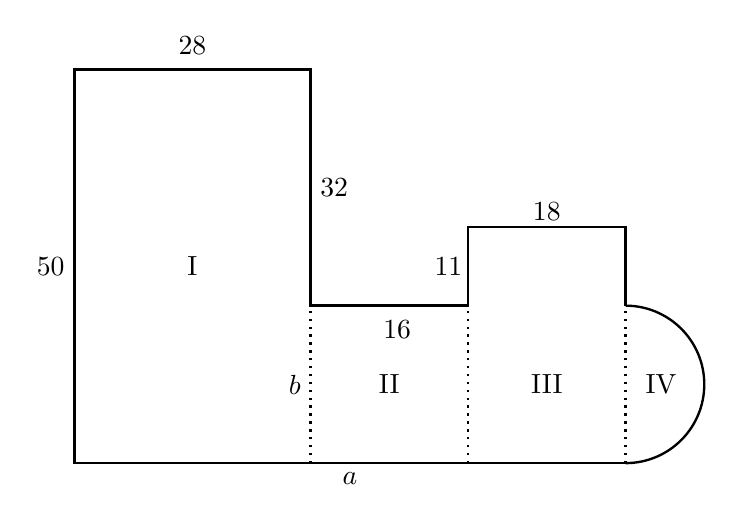
\begin{tikzpicture}
	\draw[line width=0.03cm] (7,0) -- (0,0) -- (0,5) -- (3,5) -- (3,2) -- (5,2) -- (5,3) -- (7,3) -- (7,2);
	\draw[line width=0.03cm] (7,0) arc(270:450:1);
	
	\node at (-0.3,2.5) {$50$};
	\node at (1.5,5.3) {$28$};
	\node at (3.3,3.5) {$32$};
	\node at (4.75,2.5) {$11$};
	\node at (4.1,1.7) {$16$};
	\node at (6,3.2) {$18$};
	
	\draw[line width=0.03cm,dotted] (3,0) -- (3,2);
	\draw[line width=0.03cm,dotted] (5,0) -- (5,2);
	\draw[line width=0.03cm,dotted] (7,0) -- (7,2);
	
	\node at (2.8,1) {$b$};
	\node at (3.5,-0.2) {$a$};
	\node at (1.5,2.5) {I};
	\node at (4,1) {II};
	\node at (6,1) {III};
	\node at (7.45,1) {IV};
	\end{tikzpicture}
	\]

\begin{enumerate}[(a)]
\item Find the perimeter of the region. 
\item Find the area of the region. 
\item If the region were actually the shape of a building, as viewed from above, assuming that the building is `regularly shaped', 38~ft high, and all the measurements in the figure shown above were in feet, what is the volume of the building?
\end{enumerate} \pspace

\sol First, break the region as shown above. Examining the diagram, observe that $a$ must be the length of the sum of the lengths of the `opposite' sides. But then $a= 28 + 16 + 18= 62$. Furthermore, we can see that 50 must be the same as its `opposite' sides. But then $50= 32 + b$, so that $b= 18$. Then there is a semicircle on the right side of the region with diameter 18, i.e. radius 9. 


\begin{enumerate}[(a)]
\item The perimeter of the region is the sum of the lengths of its `sides.' The only `difficult' side is the portion of the right side that is a semicircle. The perimeter of a circle is the circumference and is given by $C= \pi d$. Then the perimeter is\dots
	\[
	P= 50 + 28 + 32 + 16 + 11 + 18 + 11 + \frac{1}{2}\, \pi \cdot 18 + 62= 228 + 9\pi \approx 256.27
	\]

\item Break the region above into the regions labeled I, II, III, and IV. The regions I, II, and III are rectangles. The area of a rectangle is $A= \ell w$, where $\ell$ is the length and $w$ is the width. region~IV is a semicircle. A circle has area $A= \pi r^2$. Therefore, region~IV has area $\frac{1}{2}= \frac{\pi r^2}{2}$. But then we have\dots
	\[
	A= A_{\text{I}} + A_{\text{II}} + A_{\text{III}} + A_{\text{IV}}= 50(28) + 18(16) + (11 + 18)18 + \frac{\pi \cdot 9^2}{2}= 2210 + \frac{81 \pi}{2} \approx 2337.23
	\]

\item The building is formed from cross sections with shape given in the problem statement and height 38~ft. Recall that from Cavalier's Principle, the volume of a `prism' is the area of a cross section, $A$, times its height, $h$. From (b), we know the area of a cross sectional area is 2337.23~ft$^2$. But then the volume of the building is\dots
	\[
	V= Ah= 2337.23 \text{ ft}^2 \cdot 38 \text{ ft}= 8,\!8814.74 \text{ ft}^3
	\]
\end{enumerate}

\newpage 

{\itshape Note. One could do (c) as follows: break the region into the regions labeled in the diagram---as in the start of the problem. Then viewing the building as consisting of these regions, we know that $V_{\text{building}}= V_{\text{I}} + V_{\text{II}} + V_{\text{III}} + V_{\text{IV}}$. Three-dimensionally, regions I, II, and III are rectangular prisms. The volume of a rectangular prism is $V= \ell w h$, where $\ell$ is the length, $w$ is the width, and $h$ is the height. But then we have\dots
	\[
	\begin{aligned}
	V_{\text{I}}&= \ell w h= 50 \text{ ft} \cdot 28 \text{ ft} \cdot 38 \text{ ft}= 53,\!200 \text{ ft}^3 \\
	V_{\text{II}}&= \ell w h= 16 \text{ ft} \cdot 18 \text{ ft} \cdot 38 \text{ ft}= 10,\!944 \text{ ft}^3 \\
	V_{\text{III}}&= \ell w h= 18 \text{ ft} \cdot (11 \text{ ft} + 18 \text{ ft}) \cdot 38 \text{ ft}= 18 \text{ ft} \cdot 29 \text{ ft} \cdot 38 \text{ ft}= 19,\!836 \text{ ft}^3 
	\end{aligned}
	\]
Observe that region~IV will three-dimensionally be a half cylinder. The volume of a cylinder is $V= \pi r^2 h$, where $r$ is the radius, and $h$ is the height. But then $\frac{1}{2}V= \frac{1}{2} \pi r^2 h$. But then we have\dots
	\[
	V_{\text{IV}}= \dfrac{1}{2} \pi r^2 h= \dfrac{1}{2} \cdot \pi \cdot \left( \dfrac{18 \text{ ft}}{2} \right)^2 \cdot 38 \text{ ft}= \dfrac{1}{2} \cdot \pi \cdot (9 \text{ ft})^2 \cdot 38 \text{ ft}= \dfrac{1}{2} \cdot \pi \cdot 81 \text{ ft}^2 \cdot 38 \text{ ft}= 1539 \pi \text{ ft}^3 \approx 4,\!834.91 \text{ ft}^3
	\]
Therefore, we know\dots
	\[
	\begin{aligned}
	V_{\text{building}}&= V_{\text{I}} + V_{\text{II}} + V_{\text{III}} + V_{\text{IV}} \\[0.3cm]
	&= 53,\!200 \text{ ft}^3 + 10,\!944 \text{ ft}^3 + 19,\!836 \text{ ft}^3 + 1539 \pi \text{ ft}^3 \\[0.3cm]
	&= 83,\!980 \text{ ft}^3 + 1539 \pi \text{ ft}^3 \\[0.3cm]
	&\approx 83,\!980 \text{ ft}^3 + 4,\!834.91 \text{ ft}^3 \\[0.3cm]
	&= 88,\!814.91 \text{ ft}^3
	\end{aligned}
	\]
This is the same answer obtained in (c)---up to rounding:
	\[
	V= Ah= \left( 2210 + \frac{81 \pi}{2} \right) \text{ ft}^2 \cdot 38 \text{ ft}= 83,\!980 \text{ ft}^3 + 1539 \pi \text{ ft}^3 \approx 88,\!814.91 \text{ ft}^3
	\]
}


\end{document}